%===============================================================================
% $Id: ifacconf.tex 19 2011-10-27 09:32:13Z jpuente $  
% Template for IFAC meeting papers
% Copyright (c) 2007-2008 International Federation of Automatic Control
%===============================================================================
\documentclass{ifacconf}

\usepackage{graphicx,times}
\usepackage{natbib}        % required for bibliography
\usepackage{xcolor}

\usepackage[utf8x]{inputenc}
\usepackage{lmodern,textcomp}
\usepackage{multirow}
%\usepackage{subfig}
%\usepackage{caption}
\usepackage{tipa}
\usepackage{graphicx}
\usepackage{hyperref}
\usepackage{multirow}
\usepackage{verbatim}
\usepackage{booktabs}
\usepackage{booktabs,siunitx}
\usepackage{amsmath}
\usepackage{amsfonts}  
\usepackage{enumitem}

%===============================================================================
\begin{document}
\begin{frontmatter}

\title{Stochastic modelled grid outage effect on a solar home} 
% Title, preferably not more than 10 words.

\author[First]{Jesse-James PRINCE AGBODJAN}
\author[First]{Pierre HAESSIG} 
\author[First]{Romain BOURDAIS}
\author[First]{Herve GUEGUEN}

\address[First]{CentraleSupelec CNRS IETR (Institut d'Electronique et de Telecommunications de Rennes), UMR 6164, F-35000 Rennes, France (e-mails : \{jesse-james.prince-agbodjan, pierre.haessig, romain.bourdais, herve.gueguen\}@centralesupelec.fr)}

\begin{abstract}                % Abstract of not more than 250 words.
This paper describes the process of introducing resilience in an existing controller based on Model Predictive control. The resulting controller called \textit{resilient controller} aims at improving energy resilience during power outages by maintaining at least a minimum level of energy set by the user. The performances of the so-called \textit{resilient controller} are compared with others controllers. The results show that the \textit {resilient controller} is capable of satisfying a settled electricity need of an energetic system as long as possible during an outages, hence improving the resilience.
\end{abstract}

\begin{keyword}
Home Energy Management System (HEMS) , Resilience, Model Predictive Control (MPC), multi objectives optimization, Open Loop Feedback Controller(OLFC)].
\end{keyword}

\end{frontmatter}
%===============================================================================

\section{Introduction}


%%
\section{Case Study}\label{Section2}

\subsection{System description}
\begin{figure}[!ht]
        \begin{center}
                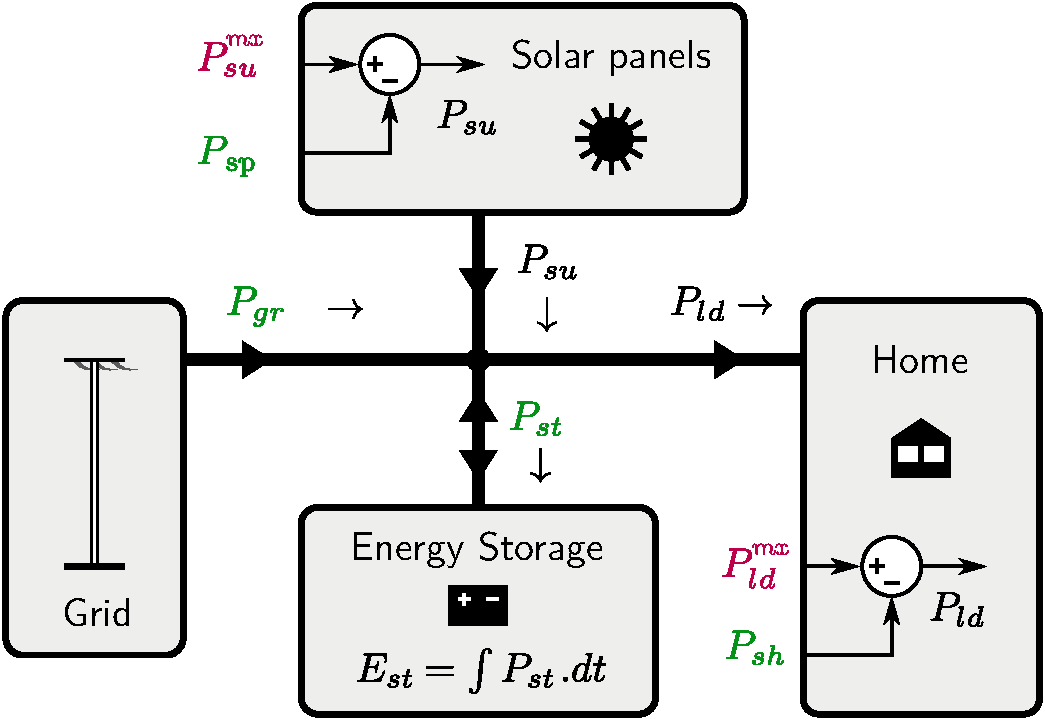
\includegraphics[width=0.9\columnwidth]{Figures/solar_home2.pdf}
        \end{center}

        \caption{Power flow model of a solar home.
        The decision/controlled variables are colored in green, external data are colored in red (Solar potential and desired consumption), internal variables are colored in black.
        }
        \label{fig:solhome}
\end{figure}
\quad The Case Study is a solar home represented by its power flow model (Fig.~\ref{fig:solhome}). It is a discrete time model of a photovoltaic system with storage for the auto-consumption of a residential consumer connected to the power grid. It is comprised of 2 externals known variables $P_{su}^{mx}$, $P_{ld}^{mx}$ respectively the solar potential production  and the power demand of the house (in red) and 4 controlled variables $P_{gr}$, $P_{cu}$, $P_{st}$ and $P_{sh}$ (in green). The optimization problem solved by the controller is define as follows: 

\section{Towards a resilient MPC }\label{section3}
The system described  is given by the following optimization: 
\begin{align} 
& \underset{P_{gr},P_{sp},P_{st},P_{sh}}{\text{min}} J = \sum_{k=1}^{N} C_{gr}P_{gr} + C_{sp}P_{sp}+ C_{sh}P_{sh} \label{eq:cost2min}\\
& \text{\hspace{20px} s.t.\hspace{15px}}  \underbrace{0 \leq P_{gr}}_{(2.a)}, \hspace{10px} \underbrace{P_{gr}\leq P_{gr}^{mx}}_{(2.b)} \label{eq:Pgr_cons} \\
& \hspace{52px} 0 \leq P_{sp} \leq P_{su}^{mx} \label{eq:Pcu_cons}\\
& \hspace{52px} 0 \leq P_{sh} \leq P_{ld}^{*} \label{eq:Psh_cons} \\
& \hspace{52px} 0 \leq E_{st} \leq E_{st}^{mx} \label{eq:Est_cons} \\
& \hspace{52px} E_{st}(k+1) = E_{st}(k) + P_{st}(k)\Delta_t \label{eq:Est_dyn}  \\
& \hspace{52px} P_{gr}- P_{st}+ \underbrace{P_{su}^{mx}-P_{sp}}_{P_{su}} =\underbrace{P_{ld}^{mx} - P_{sh}}_{P_{ld}} \label{eq:Engy_csvt} 
\end{align}
where
\begin{itemize}
\item $P_{gr}$ is the power drawn from the grid bounded bellow and above
respectively by 0 (selling energy is not authorized) and the maximum power subscribed by the user $P_{gr}^{mx}$,
\item $P_{sp}$ is the spilled \textcolor{red}{(or wasted)} solar power when it cannot be used directly or stored, $P_{su}$ the maximum solar potential and 
\item $P_{sh}$ the shedded power representing the energy not provided to the load (house), hence the actual power provided to the load $P_{ld} = P_{ld}^{mx} - P_{sh}$
\item $P_{st}$ the power into/out of the storage unit, which accumulation over time gives the energy in the battery $E_{st}$, of course constrained above by $E_{st}^{mx}$ the maximum capacity of the battery. 
\end{itemize}

Note that all the variables and constraints of the previous problem are evaluated at each instant $k \in \{1, \ldots, N \}$, i.e. should therefore been indexed by `` $k$ '' but we have deliberately choose not to  put it for clarity and simplicity sake as we will do for the rest of the paper.

Introduced in the model Predictive Control (MPC) framework, the previous problem is no longer solved over the long horizon N but rather on a sliding horizon H. It becomes : 
\begin{equation}\label{eq:MPCsys}
\left. 
\begin{aligned}
&\underset{P_{gr},P_{sp},P_{st},P_{sh}}{\hspace{10px} \text{min} \hspace{10px}J_H =} \sum_{j=k}^{k+H} C_{gr}P_{gr} + C_{sp}P_{sp}+ C_{sh}P_{sh}\\
& \text{\hspace{20px} s.t.\hspace{15px}} (\ref{eq:Pgr_cons}),(\ref{eq:Pcu_cons}),(\ref{eq:Psh_cons}), (\ref{eq:Est_cons}), (\ref{eq:Est_dyn}),(\ref{eq:Engy_csvt})
\end{aligned}\right \}
\end{equation}

If the trajectory of all the problem's inputs i.e. $P_{ld}^{mx}$, $P_{su}^{mx}  \text{ and } P_{gr}^{mx}$ are known in advance, solving it is straight because we obtain a deterministic optimization problem. 
That is the case that have been extensively  treated in \cite{JPrPHa2019}.

In the other hand consider now the case where $P_{gr}^{mx}$ is a random variable taking its value in a set $\mathcal{P}$ defined as $ \mathcal{P} = \left \{ P_0^m , P_1^m\right \}$. Note that $P^m_0=0$ and $P_1^m$ is the maximum power subscribed by the user. More Explicitly : \begin{itemize}
\item $P_{gr}^{mx} = P_0^m \rightarrow$ the grid is not available, an outage is occurring ; 
\item $P_{gr}^{mx} = P_1^m \rightarrow$ the grid is available and we can draw energy from it . 
\end{itemize}

Taking now into consideration the stochastic characteristic of $P_{gr}^{mx}$, problem (\ref{eq:MPCsys}) is ill defined since we do not have a clear definition of what constraint (2.a) means. Yet, such a definition ought to be found if we want to solve the said problem. Two optimization fields  provide a framework which give a sensible meaning to such a ``random inequality system”. These are Robust Optimization (RO) (\cite{BenTal2009}) and Probabilistic Programming (\cite{Ankopa1995}).

The \textit{worst-case-oriented} RO approach as its name indicates, to solve this problem would consider the value of the r.v. (i.e. $P_0^{m}$) that produces the worst objective cost value. This results of course in a valid robust sub-optimal solution to the problem at each instant but is not interesting to be implemented since in other words it means considering that the grid is never available which is spurious.
 
 
  Probabilistic Programming problem can be formulated using two different approaches, the $probabilistic\,/\,chance$  $constraint (CC)$ and  the multistage stochastic optimization.
  
 CC has been first introduced by \cite{AChWCo1958} and further developed in \cite{AChWCo1959,AChWCo1962,AchWCo1963}. The field received later on several contribution among which \cite{AnPre1970,Tsentai1988,APrBVi1998,RHenrion2002,RHenrion2007}. 
 Chance constraint programming deal with constraints of the form
 \begin{equation}\label{eq:CCnomform}
     \mathbb{P}[g(x,\xi)\geq 0]\geq p,
 \end{equation}
 where $x \in \mathbb{R}^n$ is the decision vector, $\xi \in \mathbb{R}^m$ a r.v. and  $g: \mathbb{R}^n \mathsf{\,x\,}\mathbb{R}^m \rightarrow \mathbb{R}^k$ a constraint mapping. The level $p \in (0,1)$ is user defined and represent the safety for the decision $x$. In other words, the constraint \eqref{eq:CCnomform} says that we wish to take a decision $x$ that satisfies the k-dimensional random inequality system $g(x,\xi)\geq 0 $ with high enough probability. An important case of constraint \eqref{eq:CCnomform} is where  $x$ and $\xi$ are not coupled through the mapping but appear separate. In this case, $g$ is then of the form $g(x,\xi) = h(x)− \widetilde{g}(\xi)$. The constraint \eqref{eq:CCnomform} can then be rewrite as:
 \begin{align}
     G(x)&:= \mathbb{P}[h(x) \geq \widetilde{g}(\xi)]\geq p \label{eq:Gdex_eq1}\\
         &:= F_\xi{h(x)}\geq p \label{eq:Gdex_eq2}
 \end{align}
 and is referred to as separable chance constraints. Note that \eqref{eq:Gdex_eq2} is \;\; obtained \; by \; considering  \;that \; $\widetilde{g} = \xi$ and \\  $\mathbb{P}[\xi \leq h(x)] = F_\xi(h(x))$, where $F$ is the $ cumulative$  $distribution function$ of $\xi$.
 When using chance constraint, an important fact is that the r.v.  is assumed to have a normal law. In our case we are in the presence of a r.v variable which have a binary (Bernoulli) distribution.
 
 \section {Model of the grid behavior}
 In this paper we are mainly interested in the behavior of the controller during an outage. To do so, the availability an non availability of the electricity grid is modeled using two frameworks which are the Bernoulli process  and the Markov Chain (MC).
 \subsection{Bernoulli process model of the electrical grid}
 The Bernoulli process is a finite sequence of identically distributed and independent (iid) r.v that can only takes two values. The probability mass function of the r.v  $P_{gr}^{mx}$ representing the state of the  grid is then given by :
  \begin{itemize}
\item $\mathbb{P}(P_{gr}^{mx} = P_0^m) = \lambda $
\item $\mathbb{P}(P_{gr}^{mx} = P_1^m)= 1-\lambda$ 
\end{itemize}
At each instant j, the probability of the grid being unavailable and available respectively are therefore given by $\lambda$ and $1-\lambda$
 \subsection{Markov Chain model of the electrical grid }
 We modeled the grid secondly by a two states Markov chain given by the following picture.
 \begin{figure}[!ht]
        \begin{center}
                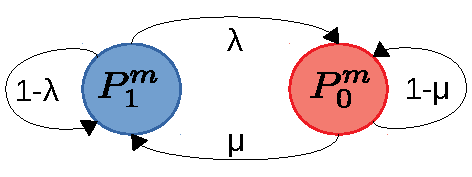
\includegraphics[width=0.65\columnwidth]{Figures/MarChain_paper.pdf}
        \end{center}

        \caption{Markov chain model of the electrical grid}
        \label{fig:MarChain}
\end{figure}

Consider that the process modelled by the different states of the electrical grid takes either the value $P^m_1$ when the grid is available or $P^m_0$ when the grid is unavailable. Let's $P^{mx}_{gr,j}$ denote its value at time period $j$. It follows that if $P_{gr,j}^{mx} = P^m_0$ or $P_{gr,j}^{mx} = P^m_1$ respectively the process is said to be in state unavailable and available at time $j$. Whenever the process is in some state, there is a fixed probability that it will be next in the another state or remains in the same. That is : 
\begin{subequations}\label{eq:MarChain}
\begin{align}
    \mathbb{P} \lbrace P^{mx}_{gr,j+1} =  P^m_0 | P^{mx}_{gr,j} = P^m_1, \ldots, X_0 \rbrace  &= \lambda, \\
    \mathbb{P} \lbrace P^{mx}_{gr,j+1} =  P^m_1 | P^{mx}_{gr,j} = P^m_1, \ldots, X_0 \rbrace  &= 1-\lambda, \\
    \mathbb{P} \lbrace P^{mx}_{gr,j+1} =  P^m_1 | P^{mx}_{gr,j} = P^m_0, \ldots, X_0 \rbrace  &= \mu, \\
    \mathbb{P} \lbrace P^{mx}_{gr,j+1} =  P^m_0 | P^{mx}_{gr,j} = P^m_0, \ldots, X_0 \rbrace  &= 1-\mu,
\end{align}
\end{subequations}

where, $X_0$, $P^{mx}_{gr,j}$ and $P^{mx}_{gr,j+1}$ represent respectively all the past states that the process has visited, the present and the future state. 

Equation (\ref{eq:MarChain}) states that, for the MC represented in Fig. \ref{fig:MarChain}, the conditional distribution of any future state $P^{mx}_{gr,j+1}$ given all the past states resumed by $X_0$ and the present state $P^{mx}_{gr,j}$ is independent of the past states and
depends only on the present state. The one step transition probabilities matrix representing the MC is then given by : 
\begin{equation}\label{eq:MarChain_TransMat}
\mathbf{P} = 
  \begin{bmatrix}
 1-\lambda  & \lambda \\ 
 \mu & 1- \mu
\end{bmatrix} . 
\end{equation}
Let's denote by $S_v^n$ the n-step state transition probability vector of the process. The \textit{Chapman–Kolmogorov equations} provide a method for computing this n-step state transition probability vector such that: 
\begin{subequations}
    \begin{align}
    S_v^n & = S_v^0 \, \mathbf{P}^n, \quad \forall n \geq 1 \label{eq:nsStaVec1} \\
          & = \bigl[ \mathbb{P} (P_{gr}^{mx} = P_1^m | S_v^0)\;\;\mathbb{P} (P_{gr}^{mx} = P_0^m | S_v^0) \bigl] \label{eq:nsStaVec2},
\end{align}
\end{subequations}
where the first and the second column of equation (\ref{eq:nsStaVec2}) represent respectively the probability of the grid being available or unavailable at time $n$ given that the initial (present) state probability vector state is $S^0_v$. At the present state we know if the electrical grid is available or not, hence $S^0_v$ taking either the value [1 0] when the grid is available and [0 1] on the contrary.

 \section{The open loop feedback controller (OLFC)}
 *Assumption: a current time all the problem variable are known even the grid i.e deterministic problem 
 Since constraint the right hand side of constraint (\ref{eq:Pgr_cons}) is  a r.v. this implies that the decision variable $P_{gr}$ is also a r.v. \\
 a way to solve this problem 
 
\begin{equation}\label{eq:Stosys}
    \underset{P_{gr},P_{cu},P_{st},P_{sh},P_{ex}}{\hspace{10px} \text{min} \hspace{10px}}  J_{OLFC},
\end{equation}
where
\begin{multline}
    J_{OLFC}  = C_{gr}(k)P_{gr}(k) + C_{cu}P_{cu}(k)+ C_{sh}P_{sh}(k) \\
                  \quad + \sum_{j=k+1}^{k+H} p_{on}(j-k)C_{gr}(j)P_{gr}(j)+p_{of}(j-k)C_{ex}P_{ex}(j) \\ + C_{sh}P_{sh}(j)+ C_{cu}P_{cu}(j)
\end{multline}


The constraint (2.a) is always satisfied so we are going to focus our attention on the constraint (2.b)

Consider problem (\ref{eq:MPCsys}) which is the minimization of the cost $J_H$ over the horizon $k$ to $k+H$. We can subdivide that problem into two phases which are the present and the future. For the present moment problem indexed by $k$, let's assume that the r.v. $P_{gr}^{mx}$ has revealed already i.e. we know which state the MC is in. In this case, dispatching the energy in each branch of the system is a simple deterministic problem. 

Now consider the future moment period ........  We are in the stochastic programming here and now framework, meaning that we need to choose how much energy must be drawn from the grid before we know if the latter is available or not. This type of problem has been extensively study in the literature under the name Newsvendor/Newsboy Inventory Problem  In we choose some value and case 

 \section{Simulation and results}
 \begin{figure}[!ht]
        \begin{center}
                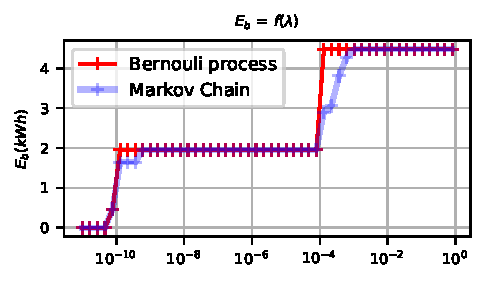
\includegraphics[width=1\columnwidth]{Figures/Mc_vs_Bp.pdf}
        \end{center}

        \caption{Comparison of the electrical grid usage for Bernoulli process and the Markov chain modeling of the grid behavior.
        }
        \label{fig:BernouVsMar}
\end{figure}
 
 
\begin{figure*}[!ht]
    \noindent  
    \begin{minipage}{.49\linewidth}
        \raggedleft
        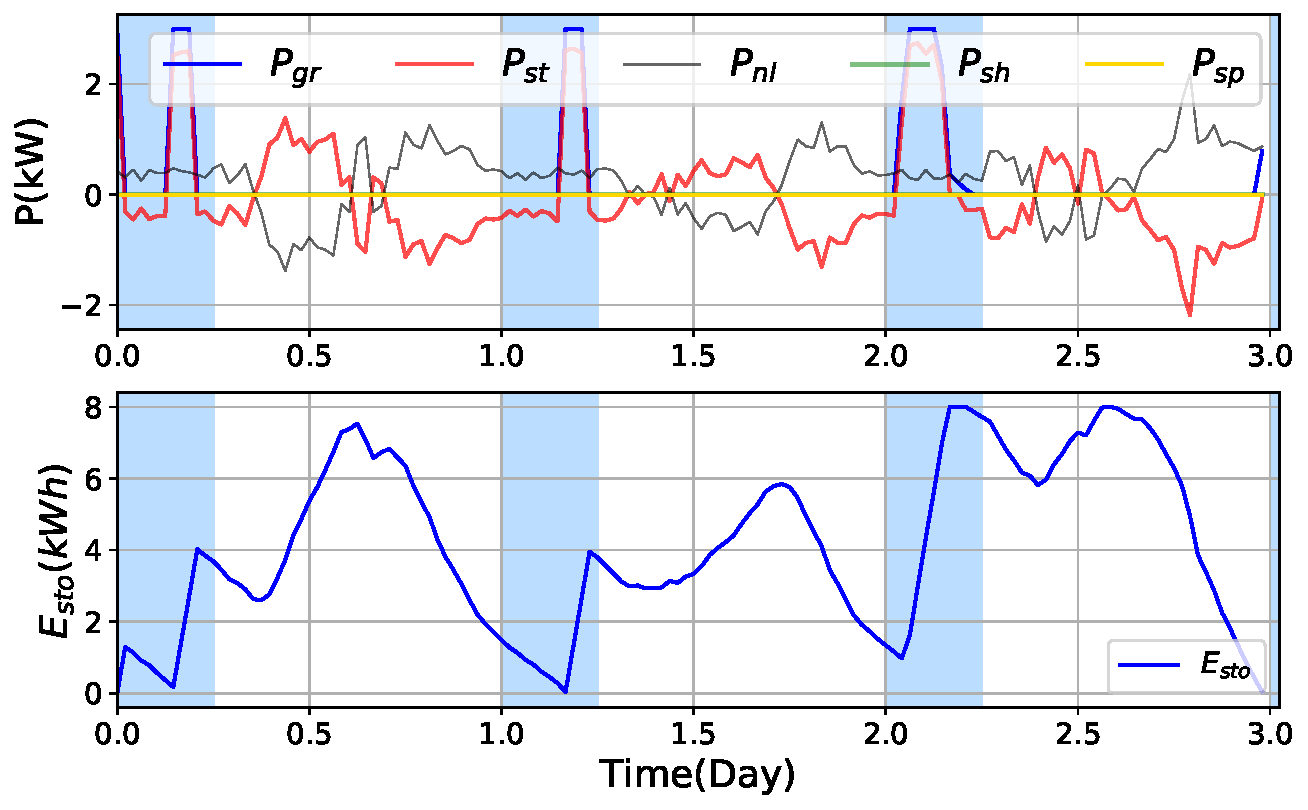
\includegraphics[height=2.5in,width=1\columnwidth]{Figures/Mc_LowFailNoOut.pdf}
        \caption{Low prob of failure, No outage}
        \label{fig:LOwFailNoOut}    
    \end{minipage}%
    \begin{minipage}{.01\linewidth}
      \hspace{1px}
    \end{minipage}%
    \begin{minipage}{0.49\linewidth}
        \raggedright
        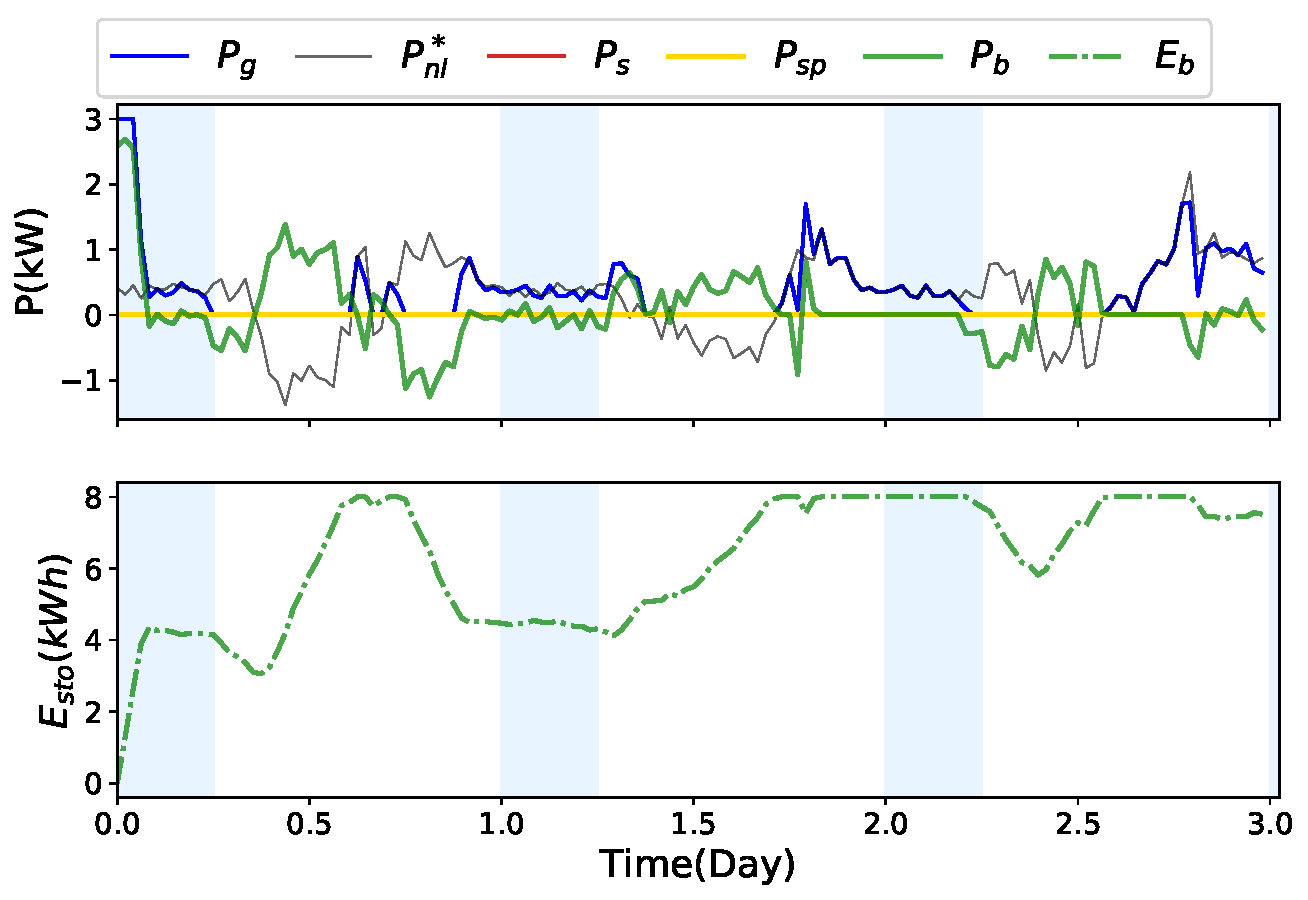
\includegraphics[height=2.5in,width=1\columnwidth]{Figures/Mc_HighFailNoOut.pdf} 
        \caption{High prob of failure, no outage}
        \label{fig:HighFailNoOut}
    \end{minipage}
\end{figure*}

\begin{figure*}[!ht]
    \noindent  
    \begin{minipage}{.49\linewidth}
        \raggedleft
        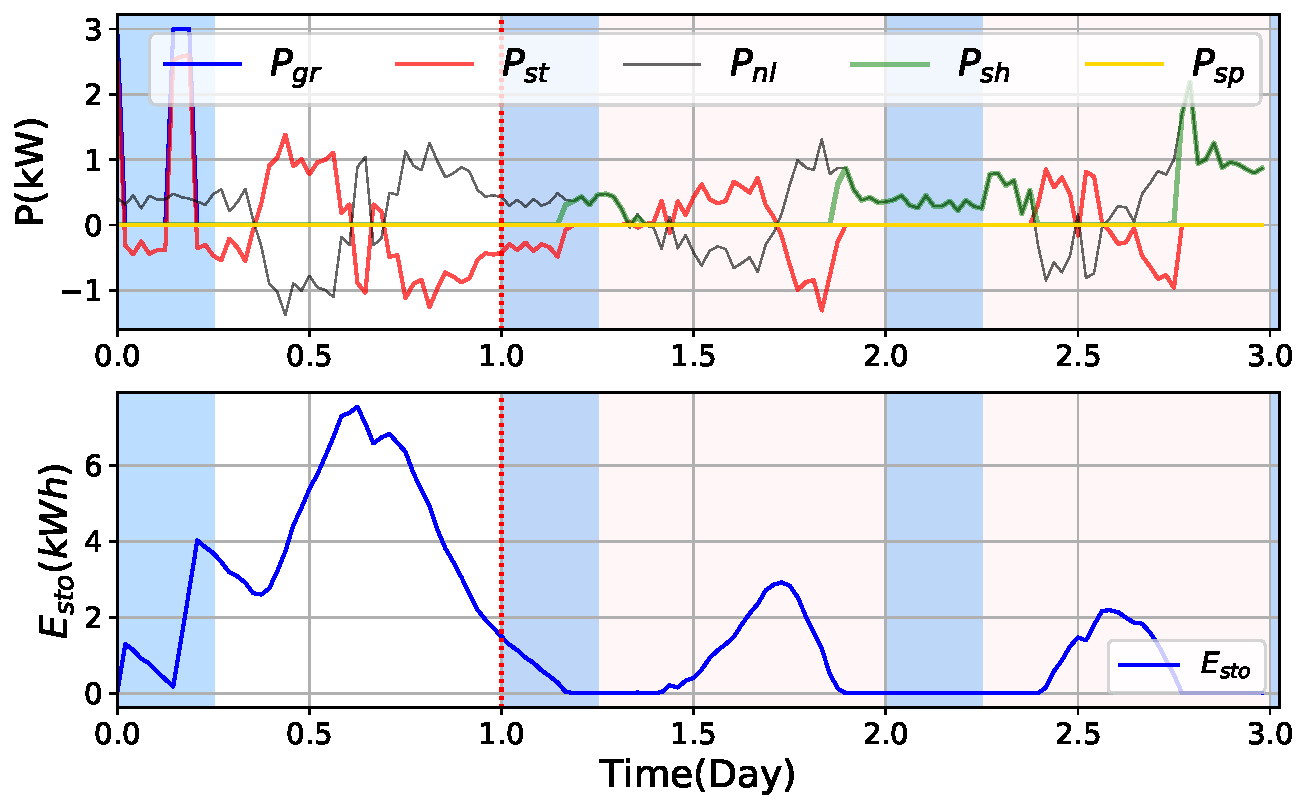
\includegraphics[height=2.2in,width=1\linewidth]{Figures/Mc_LowFailYesOut.pdf}
        \caption{Low prob of failure, with outage}
        \label{fig:LOwFailYesOut}    
    \end{minipage}%
    \begin{minipage}{.02\linewidth}
      \hspace{1px}
    \end{minipage}%
    \begin{minipage}{0.49\linewidth}
        \raggedright
        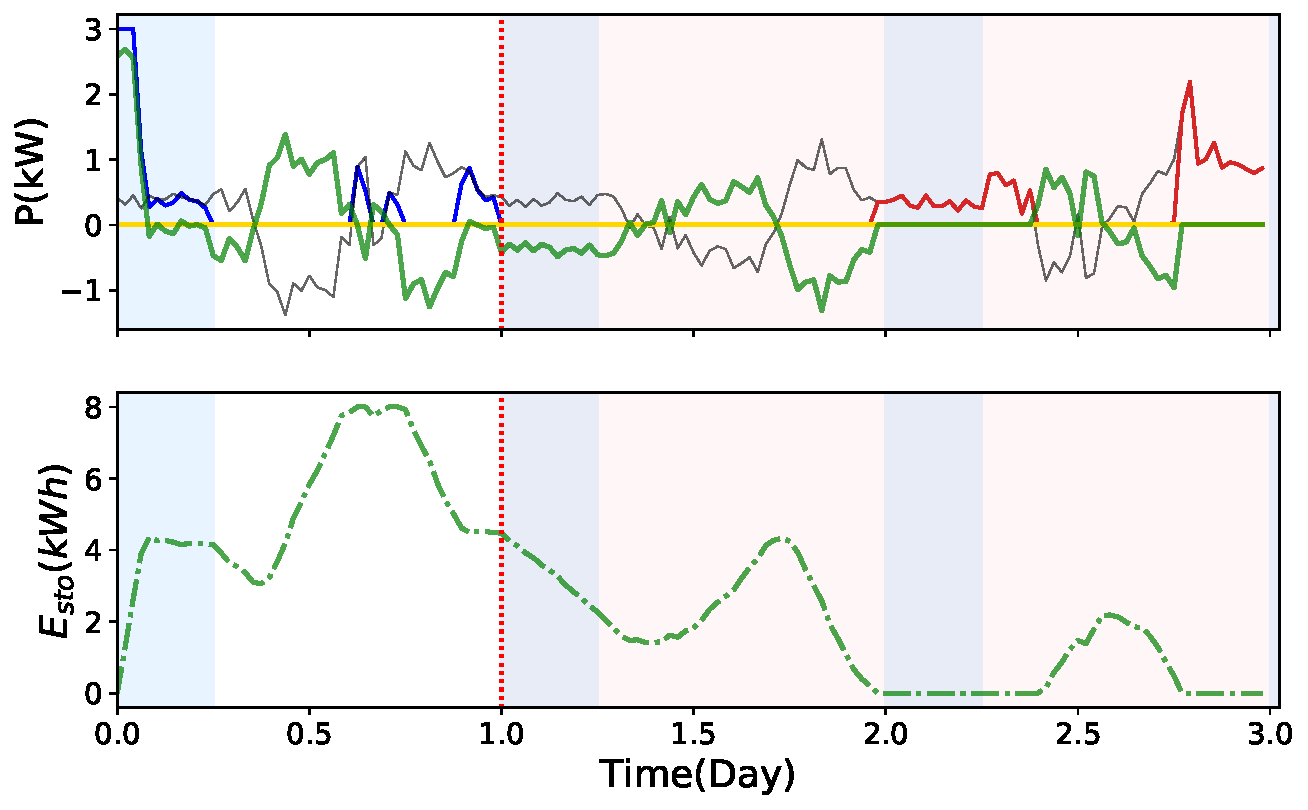
\includegraphics[height=2.2in,width=1\columnwidth]{Figures/Mc_HighFailYesOut.pdf} 
        \caption{High prob of failure, with outage}
        \label{fig:HighFailYesOut}
    \end{minipage}
\end{figure*}

\bibliography{ifac2020}
 
\end{document}

